\documentclass[10pt]{report}
\usepackage[utf8]{inputenc}
\usepackage[top=2cm, bottom=2cm, left=2cm, right=2cm]{geometry}
\usepackage[francais]{babel}
\usepackage{helvet}
\usepackage[T1]{fontenc}
\usepackage{graphicx}
\usepackage{subcaption}
\renewcommand{\familydefault}{\sfdefault}
% charte graphique non respectée pour le moment

\title{Développement d'une bibliothèque mathématique performante pour le traitement d'images médicales}
\author{Elève ingénieur : François PIAT}
\date{Année scolaire 2015-2016}

\begin{document}
	
\maketitle
\section*{Abstract/ résumé et mots-clés, Sommaire, Introduction} % dans cet ordre

\chapter{Environnement de travail} 
	\section{Le laboratoire}
	\subsection{Imperial College London - Department of computing}
%	Domaine d'activité, stats, organigramme
	\subsection{BioMedIA}
%	Synopsis, détail des activités du laboratoire
	
	La mission du groupe BioMedIA est de développer de nouvelles techniques de
	calcul pour l'analyse d'images biomédicales. Le groupe se concentre sur des
	domaines de recherche de pointe, y compris:

	- Le développement d'algorithmes d'acquisition, d'analyse et d'interprétation
	des images. En particulier dans les domaines du recalage, de la reconstruction,
	du suivi de mouvement, de la segmentation et de la modélisation.

	- L'apprentissage machine pour l'extraction d'information clinique à partir
	d'images médicales. Les applications incluent le diagnostic assisté par
	ordinateur, la planification automatisée de traitement médicale, ou encore les
	interventions et la thérapie guidées par ordinateur.

	Nous nous intéressons particulièrement à l'imagerie et les technologies de
	traitement informatique qui nous permettent de mieux comprendre le
	développement du cerveau humain, l’évolution des maladies mentales et le
	diagnostic des patients atteints de maladie cardiovasculaire.

	\section{Cadre du projet} % présentation de MIRTK, de ses applications, de son architecture(modules, fonctions...).
	 - logiciel de traitement d'image médicales, utilisé par les chercheurs en milieu médical.
	 - stable mais nécessite une maintenance et une amélioration continue pour rester pertinent.
	 Intervention sur le module "Numerics", bibliothèque mathématique.
\chapter{Objectifs et cahiers des charges}
	\section{Problématique} %Inclure contexte du projet, avec la raison pour laquelle ce projet est nécessaire.
	(back-end math) dépendances externes : eigen et boost + noyaux internes implémentés via TBB => inconsistence => parrallélisation existante floue , efficacité = ? performances=? => profilage
	===> n'utiliser qu'une seule dépendance (externe) : ArrayFire qui peut amener l'optimisation via GPU (résumer ça en 3 points majeurs)
	
	
	 

	\section{Cahier des charges}
%	Lister les attentes et les contraintes du projet.
	Arrayfire a été choisi pour palier les 3 points de la problematique \newline
	- Intégrer ArrayFire à MIRTK, aussi bien au niveau des manipulations mathématiques qu'à celui de la programmation parallèle.
	\newline- Enlever toute dépendance de MIRTK à TBB
	\newline- (Le délivrable sera composé IDEALEMENT de 2 backends, l'un AF et l'autre EIGEN. En fonction des applications, un switch automatique entre chaque structure sera appelé en dur grâce à des commandes pré-proc.) => étape bonus
	\newline- La programmation sera réalisée de manière transparente, c'est-à-dire que MIRTK doit réaliser les mêmes fonctions et garder la même API même si le code plus en profondeur est modifié.
	\newline- Plusieurs benchmarks affirmeront les performances d'ArrayFire et de l'optimisation globale de MIRTK. (test CPU et GPU)
	
	\section{Objectifs et milestones}
	
	\subsection{Objectifs} 
%	Détailler les objectifs a atteindre idéalement.
	- Ajouter ArrayFire à MIRTK, en remplaçant les fonctions d'EIGEN les moins adaptées par les fonctions d'AF. \newline
	- Faire un profiling des fonctions concernées par TBB, et interpréter les résultats afin d'élaborer une stratégie pour implanter la programmation // d'AF.\newline
	- Supprimer er les TBB inutiles ou peu efficaces, et remplacer les autres par l'équivalent d'AF (gfor).\newline
	
	
	\subsection{Diagramme de GANTT}
	 => gantt chart prévisionnel (à mettre en français)
	\begin{figure}[h!]
		\begin{center}
			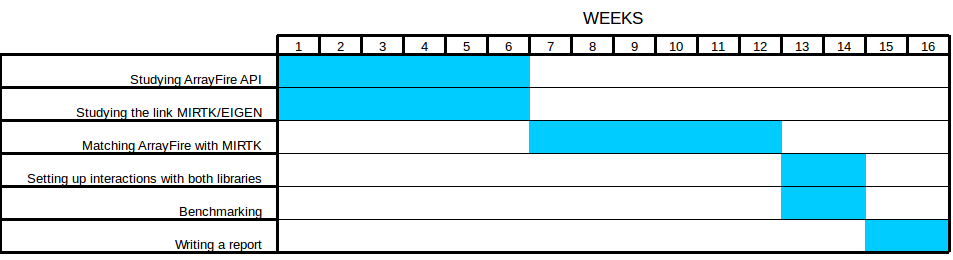
\includegraphics[width=18cm]{Reports/figures/estimated_gantt.png}
		\end{center}	
		\caption{Diagramme de GANTT prévisionnel}
		\label{Diagramme de GANTT prévisionnel}
	\end{figure}
\chapter{Réalisation}
	\section{Profilage}
%	Définir le profilage et expliquer la nécessité d'une telle étape dans ce contexte\newline
	Lors du début de mon stage, il a fallu que je me familiarise avec les dépendances de MIRTK, mais aussi a son fonctionnement interne. C'est lors de cette étude préliminaire que mon tuteur et moi avons étudié, en plus de la bibliothèque EIGEN (destinée aux fonctionnalité mathématiques), la bibliothèque "Threading Building Blocks" (abrégée TBB), qui a pour but de mettre en place une parallélisation d'un logiciel. Constatant qu'ArrayFire était constitué de fonctions mathématiques déjà optimisées sur ce plan, il a été convenu de faire un profiling de MIRTK avant d'y intégrer ArrayFire afin de prioriser les points les plus coûteux en ressources de MIRTK. 
	
	\textit{Le profilage (ou "profiling" en anglais) d'un logiciel est une évaluation des performances de celui-ci. Plusieurs critères peuvent être analysés (temps d'exécution, nombre d'instructions atomiques, fuites de cache...) et le profilage peut s'appliquer sur un fichier exécutable, ou sur un fichier source, ce qui laisse la possibilité d'analyser différentes fonctions d'un même logiciel séparément.}\\
	
	=> on identifie les fonctions sur lesquelles agir en premier
	On utilise Valgrind, qui, avec callgrind analyse la manière dont les caches sont utilisés.
%	Expliquer le choix de valgrind, parmi les autres profileurs
 => projet open-source multi-plateforme et disponible dans les packages linux, autres alternatives étudiées (VTUNE intel, installation compliquée, et codeXL, qui nécessite des proc AMD).\\
	
	
	Les tests ont été effectués sur une machine dont les caractéristiques sont les suivantes : \newline
	{$\bullet$} \textit{Nombre de coeurs:} 8, 2 threads chacun\newline
	{$\bullet$} \textit{Cadence:} 1.6 GHz \newline
	{$\bullet$} \textit{Nombre de caches:} 4 \newline
	{$\bullet$} \textit{Taille des caches:}32k, 32k, 256K, 8192K \newline
	ajouter le maximum de détails (RAM, nom du proc ...)\newline
	Pour une quantité réduite de tests, et afin de cibler les modèles d'utilisation de TBB à remplacer, on a pris l'une des fonctions les plus sollicitées dans MIRTK, il s'agit d'une fonction nommée \textit{transform-image}, et qui dispose de 5 options, définissant un type d'interpolation mathématique : Linéaire (par défaut), méthode voisin le plus proche (NN), gaussienne, sinus cardinal et B-Spline. 
	
	\subsection{Analyse du nombre d'instructions}
	
	Placer ici des graphiques de performances, avec leurs interprétation
	\subsection{Analyse des fuites de cache}
	
	Placer ici des graphiques des fuites de cache, avec leurs interprétation
	
	\section{Integration d'ArrayFire dans MIRTK}
	\subsection{Implémentation du module mathématique}
%	Programmation transparente entre Eigen et ArrayFire.
%	Lister les fonctions principales à substituer.
	\subsection{Gestion de la programmation parallèle}
%	Optimisation des threads et suppression de TBB au profit de ArrayFire.
%	\newline
%	Le contenus des sous-parties, ainsi que d'éventuelles d'autres sous-parties dépendront du résultat du profilage.
	\subsection{Switch automatique de back-end}
%	Commandes prépocesseur pour indiquer au logiciel quel est le back-end à utiliser (ArrayFire ou Eigen) en fonction de l'opération souhaitée.
	\section{Benchmarking}
	(partie dépendante du déroulement du projet)\newline
	- Analyse des performances obtenues \newline
	- Comparaison avec le profilage initial ? \newline
	- Points où il y a eu des concessions (exemple: alourdir le code pour parvenir à un résultat précis)
	
	\section{Améliorations et perspectives}
	
\section*{Conclusion, Sources, Table des illustrations, Glossaire, Annexes} % dans cet ordre
	
\end{document}
